\documentclass[11pt, twocolumn]{article}

\usepackage[spanish]{babel}
\usepackage[none]{hyphenat}
\usepackage[left=1.5cm, right=1.5cm, top = 2cm, bottom=2.5cm]{geometry}
\usepackage{parskip}
\usepackage[export]{adjustbox}
\usepackage{enumitem}
\usepackage{listings}
\usepackage{color}
\usepackage{fancyhdr}
\usepackage{graphicx}
\usepackage{caption}
% \usepackage{subcaption}
% \usepackage{wrapfig}
\usepackage{longtable}
\usepackage{multirow, makecell}
% \usepackage{amsmath} 
% \usepackage{amsfonts}
\usepackage[hidelinks]{hyperref}
\usepackage{csquotes}

\newcommand{\linejump}{\hfill \break}
\renewcommand{\thefootnote}{\fnsymbol{footnote}}
% \newcommand{\unit}[1]{\ensuremath{\, \mathrm{#1}}}

\definecolor{dkgreen}{rgb}{0,0.6,0}
\definecolor{gray}{rgb}{0.5,0.5,0.5}
\definecolor{mauve}{rgb}{0.58,0,0.82}
\lstset{
  language=Java,
  aboveskip=3mm,
  belowskip=3mm,
  showstringspaces=false,
  columns=flexible,
  basicstyle={\tiny\ttfamily},
  numbers=none,
  numberstyle=\tiny\color{gray},
  keywordstyle=\color{blue},
  commentstyle=\color{dkgreen},
  stringstyle=\color{mauve},
  breaklines=true,
  breakatwhitespace=true,
  tabsize=2
}

\sloppy
\setlength{\parindent}{0cm}
\setlength{\columnsep}{0.5cm}
\decimalpoint
\graphicspath{{img/}}

\hypersetup{colorlinks=true, urlcolor=blue, citecolor=blue}
\urlstyle{same}

\pagestyle{fancyplain}
\fancyhf{}
\fancyhead[L]{\scriptsize 
  Universidad Nacional Autónoma de México \\
  Laboratorio de Programación Orientada a Objetos \\
  M.C. Leonardo Ledesma Dominguez
}
\fancyhead[R]{\thepage}


\begin{document}
  \twocolumn[
    \centering
    Acosta Porcayo Alan Omar, Gutiérrez Grimaldo Alejandro, Medina Villa Samuel

    \linejump

    \LARGE \textbf{Práctica 8. Polimorfismo} \\
    
    \linejump
  ]
      
  \footnotetext{
    \scriptsize 
    Acosta Porcayo Alan Omar Ing. en Computación 320206102 \\
    Gutiérrez Grimaldo Alejandro Ing. en Computación 320282098 \\
    Medina Villa Samuel Ing. en Computación 320249538
  }
        
  \fancyfoot{}

  \section*{Resumen}
  En esta práctica se implementa el concepto de polimorfismo a través de una jerarquía de clases. Se crean referencias que pueden comportarse como diferentes objetos dentro de esta jerarquía. Se diseñan métodos polimórficos que permiten a las referencias acceder a comportamientos específicos de cada subclase. Esto demuestra la flexibilidad y extensibilidad que el polimorfismo aporta al código, permitiendo la interacción uniforme con objetos diversos. En resumen, la práctica destaca la importancia del polimorfismo como una herramienta clave en la programación orientada a objetos para mejorar la modularidad y escalabilidad del software.

  \section*{Introducción}
  \subsection*{Polimorfismo}
  El polimorfismo es un pilar esencial de la programación orientada a objetos. Su nombre proviene del griego y significa "muchas formas". En este contexto, se refiere a la capacidad de enviar mensajes sintácticamente iguales a objetos de tipos distintos. Esto implica que un objeto de una clase puede comportarse como un objeto de cualquiera de sus subclases.

  El polimorfismo se puede aplicar tanto a métodos como a tipos de datos. Los métodos pueden evaluarse y aplicarse a diferentes tipos de datos de manera indistinta. Los tipos polimórficos son tipos de datos que contienen al menos un elemento cuyo tipo no está especificado. Existen dos clasificaciones principales del polimorfismo:

  \begin{itemize}
    \item \textbf{Polimorfismo dinámico:} En este enfoque, no se especifica el tipo de datos sobre el que se trabaja, lo que permite recibir y utilizar todo tipo de datos compatibles. También se conoce como programación genérica.
    \item \textbf{Polimorfismo estático:} En este caso, se deben especificar de manera explícita los tipos de datos que se pueden utilizar antes de utilizarlos.
  \end{itemize}

  \subsection*{Clases Abstractas}
  Las clases abstractas son modelos que no pueden crear objetos debido a que definen la existencia de métodos, pero no su implementación. Algunas características de las clases abstractas incluyen:

  \begin{itemize}
    \item Pueden contener métodos abstractos (sin implementación) y métodos concretos.
    \item Pueden contener atributos.
    \item Pueden heredar de otras clases.
    \item Para declarar una clase abstracta en Java, se utiliza la palabra reservada ``\textit{abstract}'' antes de la palabra ``\textit{class}''.
  \end{itemize}

  \subsection*{Interfaces}
  Las interfaces son clases abstractas puras, lo que significa que todos los métodos en una interfaz son abstractos (sin implementación). Algunas características de las interfaces incluyen:

  \begin{itemize}
    \item Todos los métodos son siempre públicos y abstractos.
    \item	Pueden contener atributos que son públicos, estáticos y finales.
    \item	Las clases que implementan una interfaz deben definir (implementar) los métodos declarados en la interfaz.
    \item	Las interfaces pueden heredar de otras interfaces y permiten la herencia múltiple.
  \end{itemize}

  \subsection*{Implementación Múltiple}
  Una clase puede implementar varias interfaces, y se requiere que la clase implemente todos los métodos de las interfaces que se incluyan.

  \subsection*{Herencia Múltiple entre Interfaces}
  Las interfaces pueden heredar de otras interfaces, permitiendo la herencia múltiple de interfaces. La clase que implementa una interfaz que hereda de otras interfaces debe definir los métodos de todas las interfaces.

  \subsection*{Atributos en las Interfaces}
  En las interfaces, todos los atributos son públicos, estáticos y finales. Estos atributos se utilizan comúnmente para definir constantes que pueden ser accedidas sin crear objetos.
  
  Esta información proporciona una comprensión sólida de los conceptos de polimorfismo, clases abstractas e interfaces en la programación orientada a objetos, lo que es fundamental para diseñar sistemas de software flexibles y extensibles.

  \section*{Objetivos}
  \begin{itemize}
    \item Implementar el concepto de polimorfismo en un lenguaje de programación orientado a objetos.
    \item Comprender y diferenciar entre el polimorfismo dinámico y estático, y demostrar la capacidad de aplicar ambos tipos de polimorfismo en situaciones específicas.
    \item Diseñar interfaces que definen comportamientos específicos y permiten a las clases implementar múltiples interfaces para lograr una mayor flexibilidad en la interacción entre objetos.
  \end{itemize}

  \section*{Metodología} 
  \subsection*{Ejemplo de Polimorfismo}
  \textbf{Clase \textit{}} 
  \begin{lstlisting}

  \end{lstlisting}

  \section*{Resultados}
  \subsection*{Problema 1}
  Existen otros lenguajes de programación orientados objetos tales como:

  \begin{enumerate}[label=\alph*.]
    \item KOTLIN (JetBrains /2016)
    \item DART (Google / 2011)
    \item Groovy (JCP /2003)
    \item C$\#$ (Microsoft / 2000)
    \item Python (Rossum / 1991)
  \end{enumerate}
  
  Escoja un lenguaje de programación de la lista y estudie como se presenta el polimorfismo (estático y dinámico).

  \subsection*{Problema 2}
  Traduzca el código del Reino Animal visto en clase al lenguaje seleccionado en el punto anterior y conteste las siguientes preguntas en conclusiones:

  \begin{enumerate}[label=\alph*.]
    \item ¿Qué tan transparente fue realizar dicha traducción?
    \item ¿El concepto de polimorfismo se aplica de la misma manera?
    \item ¿Se consideraría Java como el padre de estos lenguajes?
  \end{enumerate}

  \textbf{Clase \textit{}}
  \begin{lstlisting}

  \end{lstlisting}  
  
  \textbf{Ejecución}
  % \begin{figure}[ht]
  %   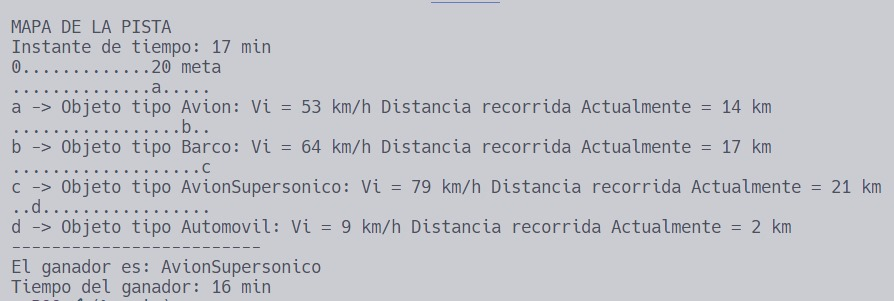
\includegraphics[width=\columnwidth, center]{P2.jpg}
  % \end{figure}

  \subsection*{Problema 3}
  Realice una tabla comparativa de desventajas y ventajas de la sobreescritura y sobrecarga de métodos y concluya desde su punto de vista cuál de las dos maneras de polimorfismo es más útil y porqué.

  
  \subsection*{Problema 4}
  Implemente la solución del siguiente problema: \url{https://edabit.com/challenge/6RStzK9uub9vHDt53}

  Pero considere la programación de los métodos polimórficos:

  \begin{enumerate}[label=\alph*.]
    \item \textit{sortByLength()} ascendente y descendente
    \item \textit{sortByAlphabet()} de a-z y z-a
  \end{enumerate}

  \textbf{Solución}
  \begin{lstlisting}

  \end{lstlisting}

  \textbf{Ejecución}
  % \begin{figure}[ht]
  %   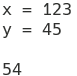
\includegraphics[width=\columnwidth, center]{P4.jpg}
  % \end{figure}

  \section*{Conclusiones}
  El polimorfismo es un concepto fundamental en la programación orientada a objetos que permite que objetos de diferentes tipos puedan interactuar de manera uniforme y eficiente. A lo largo de la información proporcionada, hemos explorado en profundidad el polimorfismo, sus tipos (dinámico y estático) y su aplicación en diferentes contextos
  
  El polimorfismo proporciona flexibilidad y extensibilidad al código, lo que es esencial para el diseño de sistemas de software versátiles y adaptables.

  Entender y aplicar de manera efectiva el polimorfismo es esencial para nosotros los programadores ya que contribuye a la construcción de software de alta calidad.


  \section*{Referencias}
  \small
  Solano, J. (2017, 20 enero). \textit{Manual de prácticas de Programación Orientada a Objetos}. Laboratorio de Computación Salas A y B. \url{http://lcp02.fi-b.unam.mx/} \\

  Zoark. \textit{Sort by Length}. Edabit. \url{https://edabit.com/challenge/6RStzK9uub9vHDt53}
\end{document}